\documentclass[10pt,a4paper,onecolumn]{article}
% \usepackage[utf8]{inputenc}
\usepackage{marginnote}
\usepackage{graphicx}
\usepackage{xcolor}
\usepackage{authblk,etoolbox}
\usepackage{titlesec}
\usepackage{calc}
\usepackage{hyperref}
\hypersetup{breaklinks=true,
            bookmarks=true,
            pdfauthor=
{
      Hrvoje Stojić,
  },
            pdftitle=
{
[Re] How learning can guide evolution
},
            colorlinks=true,
            citecolor=blue,
            urlcolor=blue,
            linkcolor=blue,
            pdfborder={0 0 0}}
\urlstyle{same}
\usepackage{tcolorbox}
\usepackage{ragged2e}
\usepackage{fontspec}
\usepackage{fontawesome}
\usepackage{caption}
\usepackage{listings}
\lstnewenvironment{code}{\lstset{language=Haskell,basicstyle=\small\ttfamily}}{}



%\usepackage{fancyvrb}
%\VerbatimFootnotes
%\usepackage{graphicx}
%\usepackage{mdframed}
%\newmdenv[backgroundcolor=lightgray]{Shaded}

% typesetting algorithms
\usepackage{algorithm}
\usepackage{algpseudocode}


\usepackage{longtable,booktabs}

\usepackage[
  backend=biber,
%  style=alphabetic,
%  citestyle=numeric
]{biblatex}
\bibliography{stojic2017.bib}



% --- Macros ------------------------------------------------------------------
\renewcommand*{\bibfont}{\small \sffamily}

\definecolor{red}{HTML}{CF232B}
\newcommand{\ReScience}{Re{\bfseries \textcolor{red}{Science}}}

\newtcolorbox{rebox}
   {colback=blue!5!white, colframe=blue!40!white,
     boxrule=0.5pt, arc=2pt, fonttitle=\sffamily\scshape\bfseries,
     left=6pt, right=20pt, top=6pt, bottom=6pt}

\newtcolorbox{repobox}
   {colback=red, colframe=red!75!black,
     boxrule=0.5pt, arc=2pt, left=6pt, right=6pt, top=3pt, bottom=3pt}

% fix for pandoc 1.14     
\newcommand{\tightlist}{%
  \setlength{\itemsep}{1pt}\setlength{\parskip}{0pt}\setlength{\parsep}{0pt}}

% --- Style -------------------------------------------------------------------
\renewcommand*{\bibfont}{\small \sffamily}
\renewcommand{\captionfont}{\small\sffamily}
\renewcommand{\captionlabelfont}{\bfseries}

\makeatletter
\renewcommand\@biblabel[1]{{\bf #1.}}
\makeatother

% --- Page layout -------------------------------------------------------------
\usepackage[top=3.5cm, bottom=3cm, right=1.5cm, left=1.5cm,
            headheight=2.2cm, reversemp, includemp, marginparwidth=4.5cm]{geometry}

% --- Section/SubSection/SubSubSection ----------------------------------------
\titleformat{\section}
  {\normalfont\sffamily\Large\bfseries}
  {}{0pt}{}
\titleformat{\subsection}
  {\normalfont\sffamily\large\bfseries}
  {}{0pt}{}
\titleformat{\subsubsection}
  {\normalfont\sffamily\bfseries}
  {}{0pt}{}
\titleformat*{\paragraph}
  {\sffamily\normalsize}


% --- Header / Footer ---------------------------------------------------------
\usepackage{fancyhdr}
\pagestyle{fancy}
%\renewcommand{\headrulewidth}{0.50pt}
\renewcommand{\headrulewidth}{0pt}
\fancyhead[L]{\hspace{-1cm}
\includegraphics[width=4.0cm]{rescience-logo.pdf}}
\fancyhead[C]{}
\fancyhead[R]{} 
\renewcommand{\footrulewidth}{0.25pt}

\fancyfoot[L]{\hypersetup{urlcolor=red}
              \sffamily \ReScience~$\vert$
              \href{http://rescience.github.io}{rescience.github.io}
              \hypersetup{urlcolor=blue}}
\fancyfoot[C]{\sffamily \thepage}
\fancyfoot[R]{\sffamily Sep 2015 $\vert$
                        Volume \textbf{1} $\vert$
                        Issue \textbf{1}}
\pagestyle{fancy}
\makeatletter
\let\ps@plain\ps@fancy
\fancyheadoffset[L]{4.5cm}
\fancyfootoffset[L]{4.5cm}

% --- Title / Authors ---------------------------------------------------------
% patch \maketitle so that it doesn't center
\patchcmd{\@maketitle}{center}{flushleft}{}{}
\patchcmd{\@maketitle}{center}{flushleft}{}{}
% patch \maketitle so that the font size for the title is normal
\patchcmd{\@maketitle}{\LARGE}{\LARGE\sffamily}{}{}
% patch the patch by authblk so that the author block is flush left
\def\maketitle{{%
  \renewenvironment{tabular}[2][]
    {\begin{flushleft}}
    {\end{flushleft}}
  \AB@maketitle}}
\makeatletter
\renewcommand\AB@affilsepx{ \protect\Affilfont}
%\renewcommand\AB@affilnote[1]{{\bfseries #1}\hspace{2pt}}
\renewcommand\AB@affilnote[1]{{\bfseries #1}\hspace{3pt}}
\makeatother
\renewcommand\Authfont{\sffamily\bfseries}
\renewcommand\Affilfont{\sffamily\small\mdseries}
\setlength{\affilsep}{1em}

\LetLtxMacro{\OldIncludegraphics}{\includegraphics}
\renewcommand{\includegraphics}[2][]{\OldIncludegraphics[width=12cm, #1]{#2}}


% --- Document ----------------------------------------------------------------
\title{[Re] How learning can guide evolution}

    \usepackage{authblk}
                        \author[1]{Hrvoje Stojić}
                            \affil[1]{Department of Economics and Business, Universitat Pompeu Fabra,
Barcelona, Spain}
            
\date{\vspace{-5mm}
      \sffamily \small \href{mailto:hrvoje.stojic@protonmail.com}{hrvoje.stojic@protonmail.com}}


\setlength\LTleft{0pt}
\setlength\LTright{0pt}


\begin{document}
\maketitle

\marginpar{
  %\hrule
  \sffamily\small
  %\vspace{2mm}
  {\bfseries Editor}\\
  Name Surname\\

  {\bfseries Reviewers}\\
        Name Surname\\
        Name Surname\\
  
  {\bfseries Received}  Aug, 20, 2017\\
  {\bfseries Accepted}  Sep, 1, 2015\\
  {\bfseries Published} Sep, 1, 2015\\

  {\bfseries Licence}   \href{http://creativecommons.org/licenses/by/4.0/}{CC-BY}

  \begin{flushleft}
  {\bfseries Competing Interests:}\\
  The authors have declared that no competing interests exist.
  \end{flushleft}

  \hrule
  \vspace{3mm}

  \hypersetup{urlcolor=white}
  
    \vspace{-1mm}
  \begin{repobox}
    \bfseries\normalsize
      \href{https://github.com/ReScience-Archives/Stojic-2017/tree/master/article}{\faGithubAlt~Article repository}
  \end{repobox}
      \vspace{-1mm}
  \begin{repobox}
    \bfseries\normalsize
      \href{https://github.com/ReScience-Archives/Stojic-2017/tree/master/code}{\faGithubAlt~Code repository}
  \end{repobox}
      \vspace{-1mm}
  \begin{repobox}
    \bfseries\normalsize
      \href{https://github.com/ReScience-Archives/Stojic-2017/tree/master/data}{\faGithubAlt~Data repository}
  \end{repobox}
      \hypersetup{urlcolor=blue}
}

\begin{rebox}
\sffamily {\bfseries A reference implementation of}
\small
\begin{flushleft}
\begin{itemize}
    \item[→] \emph{How learning can guide evolution}, G. E. Hinton, and S. J. Nowlan,
Complex Systems, 1 (3), 495-502, 1987.
  \end{itemize}\par
\end{flushleft}
\end{rebox}


\section{Introduction}\label{introduction}

The Lamarckian hypothesis that adaptations accumulated during the
lifetime of an individual organism are directly transmitted to the next
generation is considered to be incorrect. The reference article
\autocite{hinton1987learning} argues that this does not necessarily mean
that individual learning cannot exert influence on evolution in an
indirect fashion, providing a simple but convincing computational
example of such an interaction. The authors use an extreme scenario
where the optimization landscape is completely flat except for a single
peak. In such an environment, curvature of the optimization surface does
not provide any guidance and evolutionary search alone cannot find the
maximum. Through a simulation the authors show that such a hostile
environment can be tackled by a combination of evolutionary and
individual learning. In addition, if organisms can search during their
lifetime, those organisms whose genomes are closer to the targeted peak
are going to be able to find the peak with individual search. Such
organisms will have higher fitness and transmit their genes to the next
generation. In effect, capacity for individual learning ``creates a
hill'' to the peak that evolutionary search can climb, as illustrated in
Figure 1 in \textcite{hinton1987learning}\footnote{Note that captions of
  the figures are switched, caption of Figure 1 is incorrectly placed
  under Figure 2, and vice versa}. This is one of the clearest
illustrations of the benefits of individual learning for evolution and
the interaction between the two learning processes.\footnote{An indirect
  influence of individual learning on evolutionary learning is often
  called Baldwin effect.} This result has made a substantial impact in
the cognitive science literature.

The main aim of this article is to replicate the simulations reported in
the reference article \autocite{hinton1987learning}. I have corresponded
with one of the authors and learned that the original implementation of
the simulations is no longer available. I am also not aware of other
implementations elsewhere. The simulations are relatively simple, and I
thus propose a replication based on description from the reference
article. Replication code relies on R programming language \autocite{R}
and several R packages
\autocites{ggplot2}{dplyr}{reshape2}{doParallel}{foreach}{doRNG}{ggrepel}{directlabels}.

\section{Methods}\label{methods}

A description of the simulations can be found in the caption of Figure 1
in the reference article \autocite{hinton1987learning}. I consider the
description to be detailed enough for the implementation. I have
followed it closely, with two exceptions. First, I have repeated the
evolutionary search many times to average out potential noise. In the
reference article, such iterations are not explicitly mentioned, and
moreover, when interpreting their results from Figure 2, the authors
state that Figure 2 presents results of ``\ldots{} a typical
evolutionary search \ldots{}'', suggesting it is a single run of the
simulation. Second, I let the population of agents evolve for 1000
generations instead of 50 generations reported in
\textcite{hinton1987learning}. Reason for this will become clear in the
Results section.

I describe my implementation in detail in Algorithm 1. Parameters for
the simulation are summarized in Table ~\ref{tbl:parameters}.

\begin{algorithm}
\caption{Simulation description}
    \begin{algorithmic}[1]
    \For{$sim=1:noSim$}
        \State{Generate targeted genome, $g^*=\{a_i\}_{i=1}^{noAlleles}$: $a_i \sim Bernoulli(p)$, }
        \State {$p \sim Uniform(0,1)$ }
        \State{Generate initial genomes of the agents, $G=\{g_i\}_{i=1}^{noAgents}$: $\forall g_i$ generate} 
        \State {$\{a_i\}_{i=1}^{noAlleles}$ by sampling with replacement from $\{0,1,?\}$ according to $p_0,p_1,p_?$.}
        \For{$gen=1:noGenerations$}
            \For{$ag=1:noAgents$} \Comment {\textbf{Individual learning}}
                \For{$step=1:lifetime$}
                    \State {For all ? alleles in agent's genome: $a_i \sim Bernoulli(0.5)$}
                    \If{$g_i == g^*$ after individual learning} \State {\textbf{break}} \EndIf
                \EndFor
                \State {Evaluate fitness: $f_{ag} = 1 - 19(lifetime-step)/1000$}
                \State {Record frequency of Correct, Incorrect and Undecided alleles.}
            \EndFor
            \State Compute parenting probabilities: 
            \State $p_{ag}=f_{ag}/\sum_{i=1}^{noAgents}f_{i}$, $\forall ag$
            \For{$i=1:|G|$} \Comment {\textbf{Generate children genomes}}
                \State {Choose two parents by sampling with replacement according to $p_{ag}$}
                \State {Generate new genome, $g_i^{child}$: randomly choose a cross-over point, 
                \State copy all alleles from the first parent up to the cross-over point, 
                \State and from the second parent beyond the cross-over point.}
            \EndFor
            \State {Update genomes: $g_i \gets g_i^{child}$, $\forall i \in G$}
        \EndFor
    \EndFor
    \end{algorithmic}
\end{algorithm}

\hypertarget{tbl:parameters}{}
\begin{longtable}[]{@{}lll@{}}
\caption{\label{tbl:parameters}Simulation parameters. }\tabularnewline
\toprule
Table & Value & Description\tabularnewline
\midrule
\endfirsthead
\toprule
Table & Value & Description\tabularnewline
\midrule
\endhead
noSim & 100 & Number of times evolutionary search is
repeated\tabularnewline
noGenerations & 1000 & Number of generations for evolutionary
algorithm\tabularnewline
noAgents & 1000 & Number of agents in a population\tabularnewline
lifetime & 1000 & Number of cycles available for individual
learning\tabularnewline
noAlleles & 20 & Number of alleles in agent's genome\tabularnewline
\(p_0\) & 0.25 & Probability that allele is of type zero\tabularnewline
\(p_1\) & 0.25 & Probability that allele is of type one\tabularnewline
\(p_?\) & 0.50 & Probability that allele is of type ?\tabularnewline
\bottomrule
\end{longtable}

\section{Results}\label{results}

The simulation results are summarized in Figure
~\ref{fig:relFrequencies50}, which corresponds to Figure 2 from the
reference article. Qualitatively, the results are very similar - there
is an obvious increase in the proportion of alleles correctly set by the
evolutionary learning (close to 75\% by generation 50) and proportion of
incorrect alleles decreases to zero by generation 50. This is clear
evidence of individual learning guiding evolutionary search, even though
there is no direct transmission of knowledge acquired during individual
learning from one generation to the next.

\begin{figure}
\centering
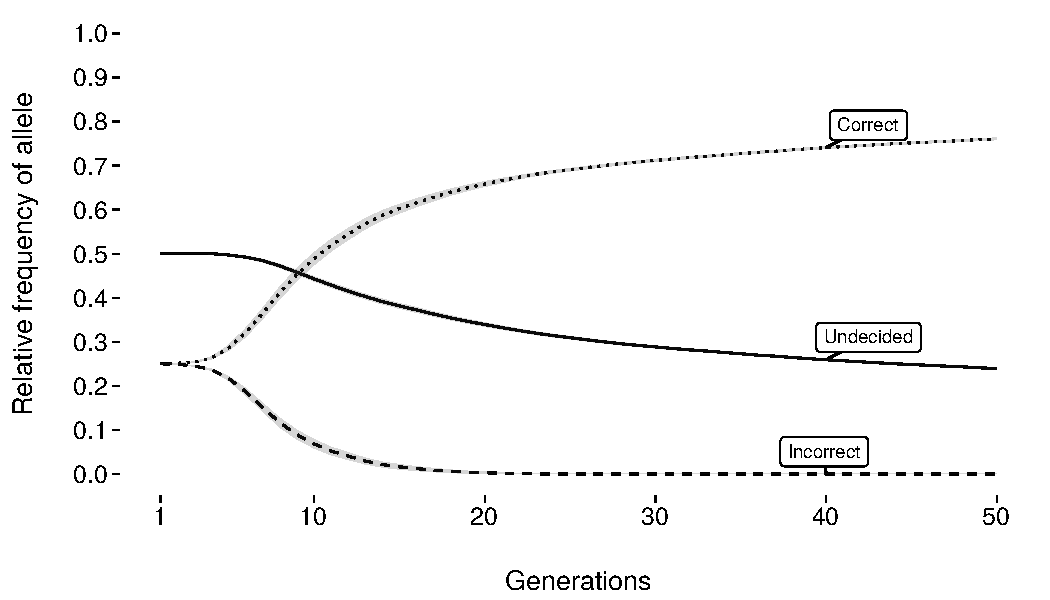
\includegraphics{Figure2.pdf}
\caption{The evolution of the relative frequencies of the three possible
types of allele. Correct alleles are those that are set by evolutionary
learning and correspond to the targeted pattern. Incorrect alleles
represent the proportion of incorrectly set alleles, while Undecided
represent the proportion of alleles left for individual learning.
Proportions are means of 100 simulation runs, and barely visible grey
ribbons are standard errors. This is the reproduction of Figure 2 in the
reference article
\autocite{hinton1987learning}.}\label{fig:relFrequencies50}
\end{figure}

There is an important difference with respect to the reference article,
however. In the original simulations, the proportion of Undecided
alleles that are left to individual learning is relatively constant,
close to initial 50\%. The authors point this out as an interesting
result, suggesting that there is little selective pressure to specify
last few connections by evolutionary learning because those can be
quickly set through individual learning. In contrast, the results in
Figure ~\ref{fig:relFrequencies50} show that the proportion of Undecided
alleles is continuously decreasing. In fact, whereas the proportion of
Correct alleles in the reference article flattens out, in my case it
continues increasing, with the increase coming from the proportion of
Undecided alleles decreasing further. To make sure that this is really a
long run trend I have let populations evolve for a larger number of
generations than in the reference article. Results of all 1000
generations are presented in Figure ~\ref{fig:relFrequencies1000}. By
generation 1000 the proportion of Undecided alleles drops to 9\%. Even
though the decrease is smaller with each generation, it does not seem to
stop and flatten out by the end of the simulation.

What is the source of this particular difference in results? One
explanation is that the results reported in Figure 2 in the reference
article stem from a non-typical draw. This is unlikely, as upon
examining the evolutionary paths of Undecided alleles in all simulation
runs, they all show a strong downward trend already in the first 50
generations, differing only in the exact generation when this decrease
onsets. Another explanation is that the original implementation is
flawed as there actually is a selection pressure for eliminating
individual learning after some time. The fitness function described in
the reference article is such that the smaller the number of steps an
agent takes in an individual lifetime to reach the peak, the higher the
probability of mating and transmitting genes to the next generation. The
number of steps is a direct function of the number of undecided alleles
in the genome. Hence, there is a selection pressure for decreasing the
number of Undecided alleles. In personal correspondence, one of the
authors agreed with this interpretation, stating that indeed there
should be a selective pressure for a decrease in number of Undecided
alleles. The pressure should decrease as a power function of the mean
number of steps an agent needs to reach the peak, which explains rapidly
decreasing improvements with each generation.

\begin{figure}
\centering
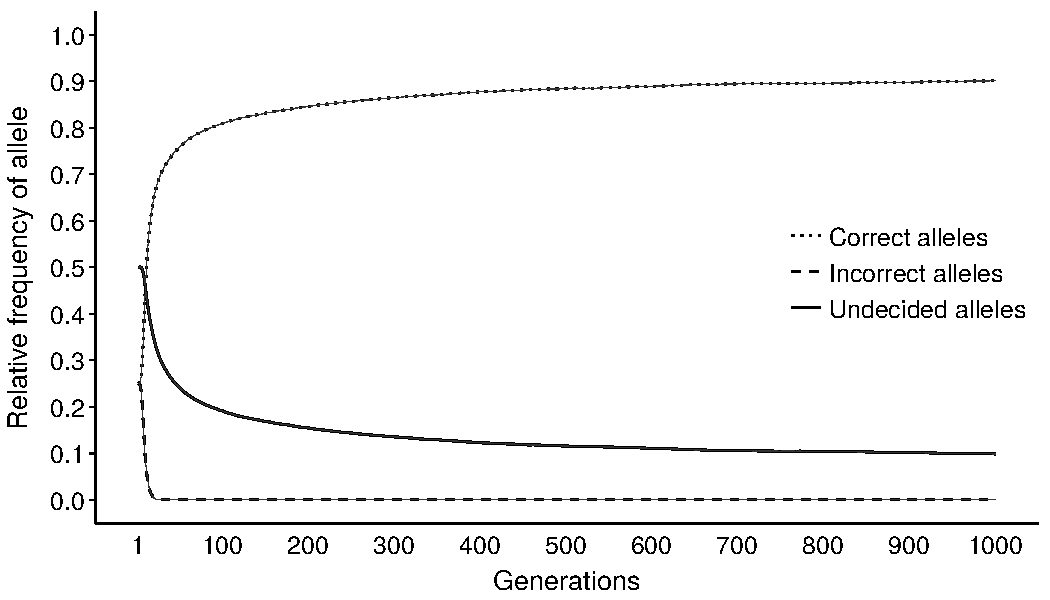
\includegraphics{Figure2_1000.pdf}
\caption{The evolution of the relative frequencies of the three possible
types of allele, with a larger number of generations. Proportions are
means of 100 simulation runs, and barely visible grey ribbons are
standard errors.}\label{fig:relFrequencies1000}
\end{figure}

\section{Conclusion}\label{conclusion}

Qualitatively, the result is comparable to that reported in the
reference article, but there are relatively important differences. The
proportion of Undecided alleles in the implementation proposed here
diminish over time, whereas in the original implementation they stay
close to the initial values. I attribute the difference to a flaw in the
original implementation, providing arguments based on a fitness function
proposed in the reference article. Although the main result of the
reference article - that individual learning can indirectly guide
evolutionary search - has been reproduced, the difference in simulation
results suggests that individual learning might be eradicated over time.
This decrease in usefulness of individual learning occurs in static
environments where targeted genome stays fixed, as in these simulations.
In more realistic scenarios, where environments are non-stationary and
the targeted genome would be changing over time, individual learning
would have a more stable role.

{\sffamily \small
  \printbibliography[title=References]
}
\end{document}
